\normaltrue \difficilefalse \tdifficilefalse
\correctionfalse

%\UPSTIidClasse{11} % 11 sup, 12 spé
%\newcommand{\UPSTIidClasse}{12}

\exer{Système de transformation de mouvement  $\star$ \label{B2:13:PTSI:13}}
\setcounter{question}{0}\UPSTIcompetence[2]{B2-13}
\index{Compétence B2-13-PTSI}
\index{Bielle Manivelle}
\index{Moteur}
\ifcorrection
\else
\textbf{Pas de corrigé pour cet exercice.}
\fi

\ifprof
\else
Soit le mécanisme suivant. 
\begin{center}
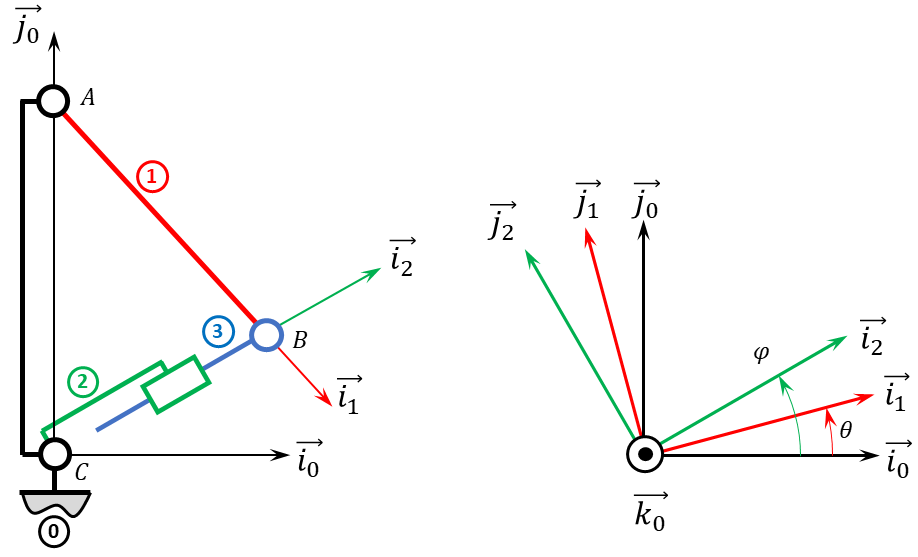
\includegraphics[width=.65\linewidth]{13_01}
\end{center}
\fi


\question{Réaliser le paramétrage du mécanisme.}
\ifprof
\else
\fi

\ifprof
\else
\begin{flushright}
\footnotesize{Corrigé  voir \ref{B2:13:PTSI:13}.}
\end{flushright}%
\fi